\section{Results}

I arbitrarily choose value function iteration when investigating the results of the model, since all the solution methods yielded identical results. 5000 agents is simulated using the optimal $\beta_L = 3.43$. Relevant summary statistics can be calculated over the 5000 simulations. The statistics can be used to infer whether or not the model fit the data and compare to what is expected from the real world. Looking to figure \ref{fig:dqi_model1_average_path_sim_vs_empirical} the empirical number of hours supplied by women \textbf{LIGEF15} is compared to the simulated. Again only women actually in the labour force  ($H>0$) is considered. The fit of the data does seem reasonable. In general the simulated data set slightly overestimates the number of supplied hours. Especially around age 30 does the simulated number of supplied hours seem to be higher than the empirical. The simulated data show heterogeneity over the life cycle, where especially the later stages of the life cycle show higher variance. This could very well stem from the idiosyncratic wage path increasing over time. Considering the estimation method relied on the number of supplied hours, it is not surprising that this is where the model performs the best. 


\begin{figure}
    \centering
    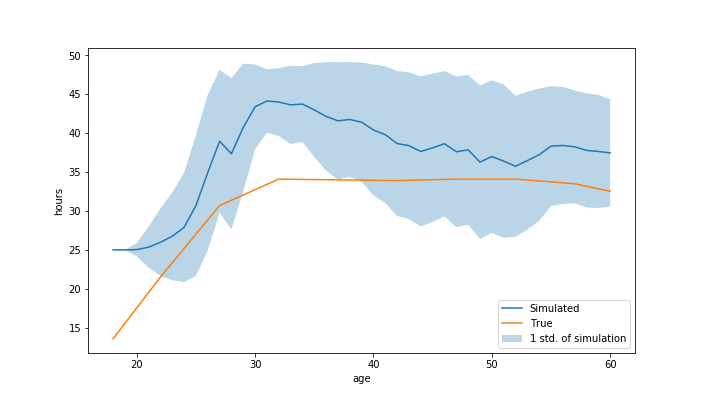
\includegraphics[scale=0.4]{figures/dqi_model1_estimation_labour_supply.png}
    \caption{Average Number of Supplied Working Hours - Empirical Vs. Simulated}
    \label{fig:dqi_model1_average_path_sim_vs_empirical}
\end{figure}

Figure \ref{fig:dqi_model1_fraction_in_workforce} shows the participation rate of women in the workforce in the simulated data set. From here it is very clear, that the model underestimates the number of women working! From age 25, 80 \% of the women is out of the workforce, followed by a slow decline in participation going forward to retirement. This does obviously not correspond to what can be observed in the real world. Even though it is not possible to get access to the exact number of women out of the labour force conditional on age, it can be approximated. Using \textbf{FOLK1B} supplied by Statistics Denmark the number of women in the age (15 to 60) can be found. Using that data the number of relevant women (considering the age) is around 1.664 million people. The number of women not working for relevant reasons can be summarized to: women not working due to: \textit{working in the home}, \textit{Studying}, \textit{Other people outside the labour force}. These add up to: $15 + 161 + 66 = 242$ thousand people or $0.242$ million people. The number of women in the relevant age group outside the labour force can be approximated to the number given in equation \ref{eq:women_outside_the_labour_force}

\begin{equation}
    \label{eq:women_outside_the_labour_force}
    \textbf{Women outside the labour force} = \frac{0.242}{1.664} = 0.145 = 14.5 \% \approx 15 \%
\end{equation}

The estimation of $\beta_L$ did not take this measure into account, which might be a way to improve the results.

\begin{figure}
    \centering
    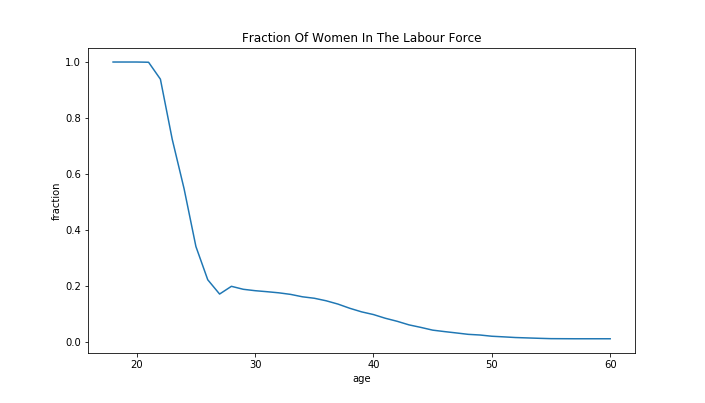
\includegraphics[scale=0.4]{figures/dqi_model1_women_in_labour_force_fraction.png}
    \caption{Fraction of Women in The Labour Force}
    \label{fig:dqi_model1_fraction_in_workforce}
\end{figure}

Both figure \ref{fig:dqi_model1_birth_onset} and figure \ref{fig:dqi_model1_child_vs_no_child_30} is inspired by the article of \textcite{kleven_children_2019}. In the article the authors show how participation of a woman is affected when she gives birth to a child. In the paper they find that women,  when giving birth to a child on average use 20 \% time less on work, compared to the husband, immediately after the birth of the child. The number of supplied hours slowly return to steady state with a long run penalty of around 6 \%. This is not the case for the simulated household. Getting a child, do seem to decrease the number of hours supplied however, the difference is indistinguishable from the mothers not getting children. This is clear in figure \ref{fig:dqi_model1_child_vs_no_child_30}, where first time mothers of age 30 is compared with women that have no children. The paths are indistinguishable, where the paper by \textcite{kleven_children_2019} would suggest a decrease of about 20 percent immediately after the birth (at age 31). These figures do not sort out women outside the labour force. I conclude the model is insufficient to capture the real world, and I move on to extend this original model.


\begin{figure}[ht]
\begin{subfigure}{.5\textwidth}
    \centering
    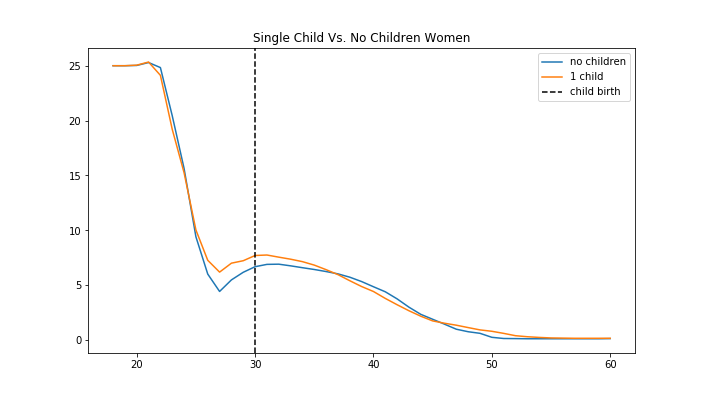
\includegraphics[width=1\linewidth]{figures/dqi_single_child_vs_no_child_model1.png}
    \caption{First time mothers vs. Women with no children}
    \label{fig:dqi_model1_child_vs_no_child_30}
\end{subfigure}%
\begin{subfigure}{.5\textwidth}
    \centering
    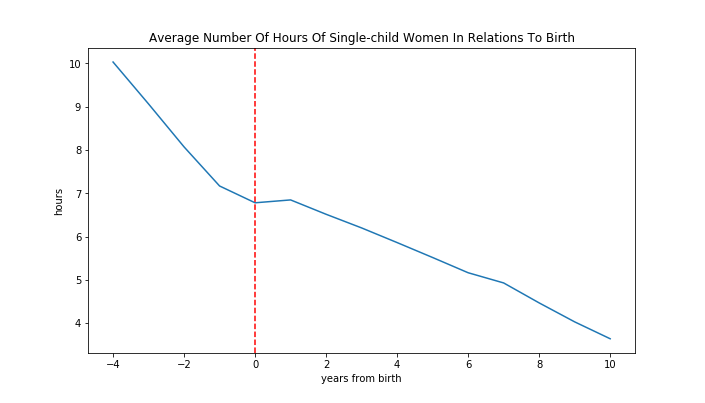
\includegraphics[width=1\linewidth]{figures/women_supplied_hours_dqi_model1_birth_onset.png}
    \caption{hours compared to birth onset.}
    \label{fig:dqi_model1_birth_onset}
\end{subfigure}
    \caption{Impact of Children}
    \label{fig:model_impact_children}
\end{figure}

